\section{User Study Additional Details}\label{app: user study}


\subsection{Data Scientist Example Workflow}

In this section we provide a detailed description of the data scientist workflow for the \userChurn task of the \handm dataset. The purpose of this is to exemplify the efforts undertaken by the data scientist to solve \relbench tasks. For data scientist solutions to all tasks, see \userstudy.

Recall that the main data science workflow steps are:
%
\begin{enumerate}
    \item Exploratory data analysis (EDA).
    \item Feature ideation.
    \item Feature enginnering. 
    \item Tabular ML.
    \item Post-hoc analysis of feature importance (optional).
\end{enumerate}



\subsubsection{Exploratory Data Analysis}

During the exploratory data analysis (EDA) the data scientist familiarizes themselves with a new dataset. It is typically carried out in a Jupyter notebook, where the data scientist first loads the dataset or establishes a connection to it and then systematically explores it. The data scientist may:
\begin{itemize}
    \item Visualize the database schema, looking at the fields of different tables and the relationships between them.
    \item Closely analyze the label sets:
        \begin{itemize}
            \item Look at the relative sizes and temporal split of the training, validation and test subsets.
            \item Look at label statistics such as the mean, the standard deviation and various quantiles. 
            \item For classification tasks, understand class (im)balance: how much bigger is the modal class than the rest? For example, in the \userChurn task roughly 82\% of the samples have label $1$, so there is a good amount of imbalance but not enough to strictly require up-sampling techniques.
            \item For regression tasks, understand the label distribution: are the labels concentrated around a typical value or do they follow a power law wherein the labels span several orders of magnitude? In extreme cases, this exploration will point to a need for specialized handing of the label space for model training.
        \end{itemize}
    \item Plot distributions and aggregations of interesting columns/fields. For example, in Figure \ref{fig:feats} we can see three such plots. From left to right:
    \begin{itemize}
        \item The first plot shows the distribution of age among customers. We see two distinct peaks one in the mid-twenties and another in the mid-fifties, suggesting different customer ``archetypes'', which may have different spending patterns.
        \item The second plot shows the number of sales per month over a two year period. We can see some seasonality with summer months being particularly good for overall sales. This suggests date related features could be useful.
        \item The third plot shows a \emph{Lorenz curve} of sales per article, showcasing the canonical \emph{Pareto Principle}: 20\% of the articles account for 80\% of the sales.
    \end{itemize}
    \item Run custom queries to look at interesting quantities and/or relationships between different columns. For instance, in the EDA for \handm, an interesting quantity to look at is the variability in item prices across the year. This reveals that most of the variability is downward, representing temporary discounts.
    \item Investigate outliers or odd-looking patterns in the data. These usually will have some real-world explanation that may inform how the data scientist chooses to pre-process the data and construct features.
\end{itemize}

In all, this process takes in the order of a few hours (3-4 for most datasets in the user study).

\begin{figure}[t]

\centering
\hspace{-40pt}
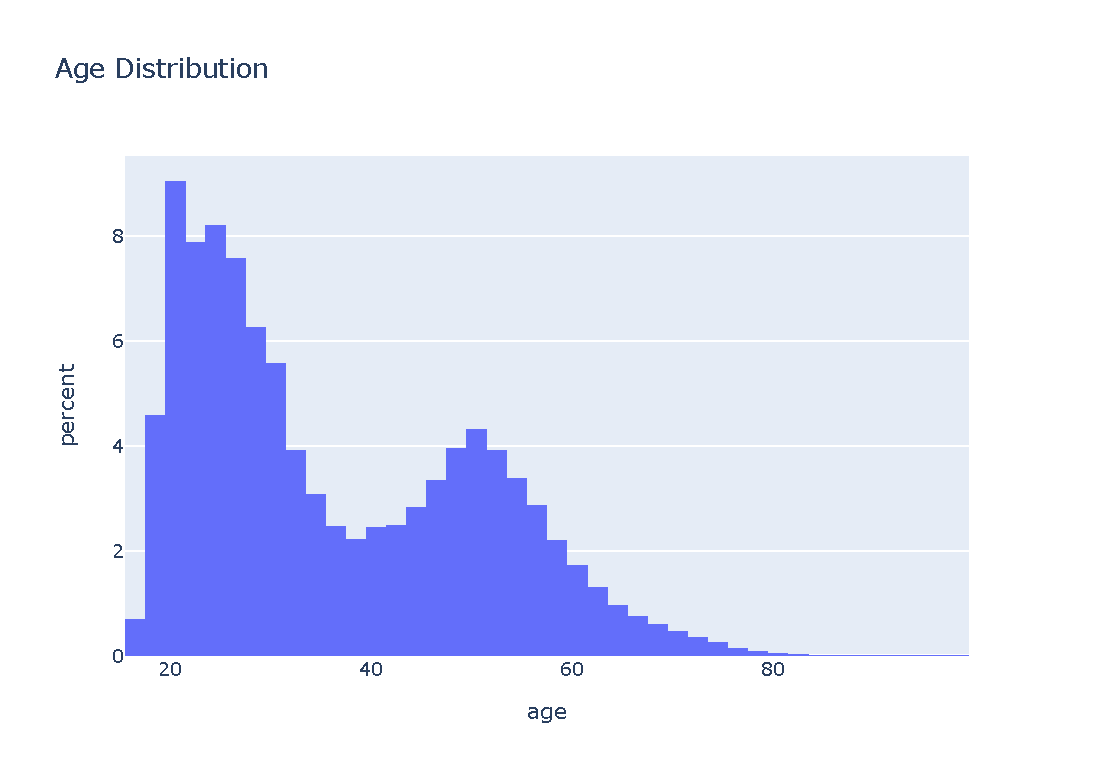
\includegraphics[width=.36\textwidth]{figs/hm_age.pdf}\hfill
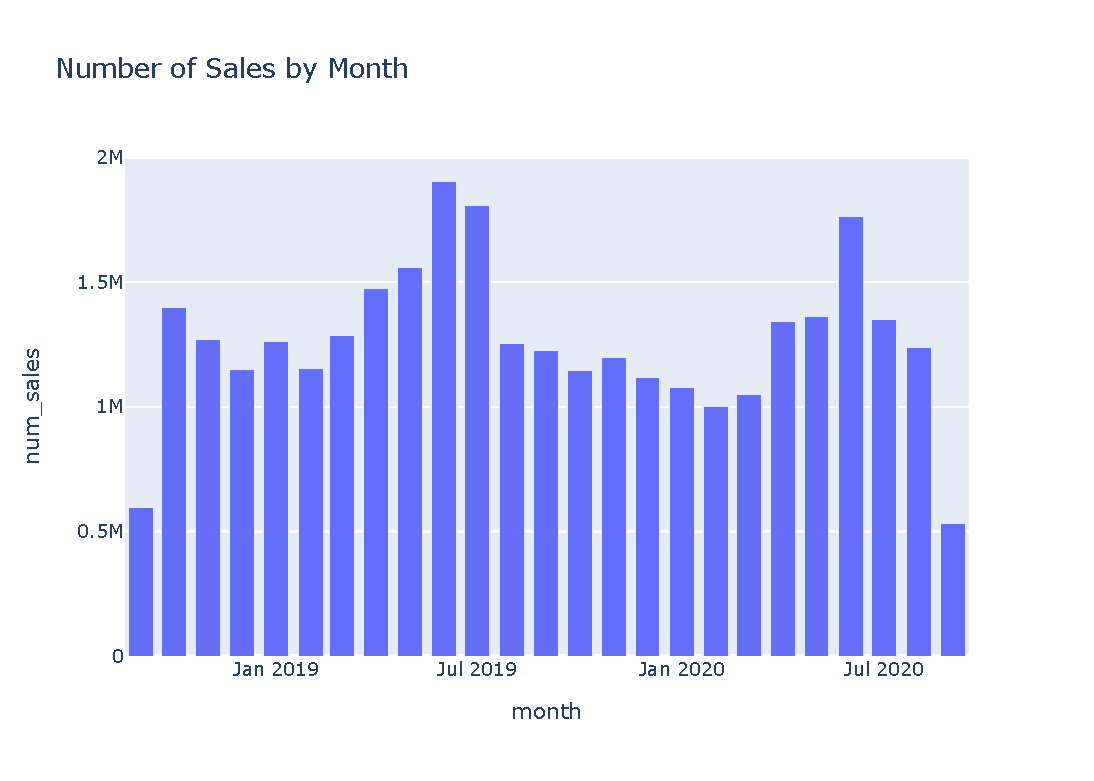
\includegraphics[width=.36\textwidth]{figs/hm_seasonality.pdf}\hfill
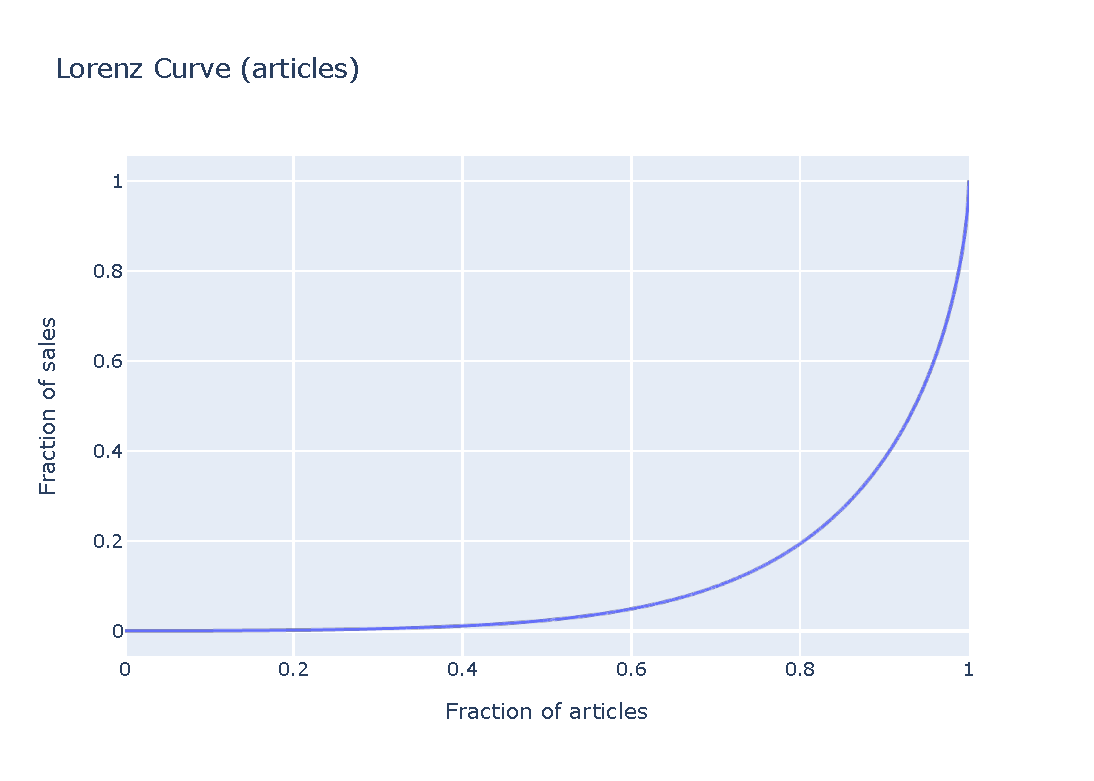
\includegraphics[width=.36\textwidth]{figs/hm_sales.pdf}
\hspace{-40pt}

\caption{\textbf{EDA Plots.} Each plot explores different characteristics of the dataset. Understanding the data and identifying relationships between different quantities is an essential prerequisite to meaningful feature engineering.}
\label{fig:feats}

\end{figure}

\subsubsection{Feature Ideation}

Having explored the dataset in the EDA, the data scientist will then brainstorm features that, to their judgement, will provide valuable signal to a model for a specific learning task. In the case of the \userChurn task, a rather simple feature would be the customer's age, which is a field directly available in one of the tables. A slightly more complex feature would be the total amount spent by the customer so far. Finally, an example of a fairly complex feature is the average monthly sales volume of items purchased by the customer in the past week. A high value for this feature may indicate that the customer has been shopping trendy items lately, whereas a low value for this feature may indicate that the customer has been interested in more arcane or specific items.

In practice, the ideation phase consists of writing down all of these feature ideas in a file or a piece of paper. It is the quickest part of the whole process and in this user study took between 30 minutes and one hour.

\subsubsection{Feature Engineering}

With a list of features in hand, the data scientist then proceeds to actually write code to generate all the features for each sample in the the train, validation and test subsets. In this user study, this was carried out using DuckDB SQL\footnote{See \url{https://duckdb.org/}.} with some Jinja templating\footnote{See \url{https://jinja.palletsprojects.com/en/3.1.x/intro/}.} for convenience.

Revisiting the example features from the previous section, the conceptual complexity of the features closely tracks with the technical complexity of implementing them. For customer age all that is required is a simple \textit{join}. The total amount spent by the customer, can be calculated using a \textit{group by} clause and a couple of \textit{join}'s. Lastly, calculating the average monthly sales volume of items purchased by the customer in the past week requires multiple \textit{group by}'s, \textit{join}'s, and \textit{window functions} distributed across multiple \textit{common table expressions} (CTEs).

A key consideration during feature engineering is the prevention of \textit{leakage}. The data scientist must ensure that none of the features accidentally include information from after the sample timestamp. This is especially true for complex features like the third example above, where special care must be taken to ensure that each \textit{join} has the appropriate filters to comply with the sample timestamp. 

For some tasks, \emph{e.g.}, \studyOutcome, the initial features \emph{did} leak information from the validation set into the training set. Thanks to the \relbench testing setup, leaking test data into the training data is hard to do by accident, since test data is hidden. Leaking information from validation to train (but not test to train) led to extremely high validation performance and very low test performance (test was significantly lower than LightGBM with no feature engineering). The large discrepancy between validation and test performances alerted the data scientist to the mistake, and the features were eventually fixed. This example illustrates another complexity that feature engineering introduces, with special care needed to ensure leakage does not happen. 

Other considerations that the data scientist must keep in mind during development and implementation of the features are parsing issues, runtime constrains and memory load. For example, during the user study we identified a parsing issue arising from special characters in user posts/comments in the \stackex dataset. The \textit{backslash} character, widely used \LaTeX can trip up certain text parsers if not handled with care. Furthermore, runtime and memory constraints are important to keep in mind when working with larger datasets and computing features that require nested \textit{join}'s and aggregations. During the user study, there were some cases where we had to refactor SQL queries to make them more efficient, increasing the overall implementation time. For some tasks we had to implement sub-sampling of the training set to reduce the burden on compute resources.

Finally, once the features have been generated for each data subset, the data scientist will usually inspect the generated features looking for anomalies (e.g. an unusual prevalence of \textit{NULL} values). In this user study we also implemented some automated sanity checks to validate the generated features beyond manual inspection.

\subsubsection{Tabular Machine Learning}

The output of the Feature Engineering phase is a DuckDB table with engineered features for each data subset. There is some non-trivial amount of work required to go from those tables to the numerical arrays used for training by most Tabular ML models (LightGBM in this case). This is implemented in a Python script that loads the data, transforms it into arrays and carries out hyperparameter tuning. In this user study we ran 5 hyperparameter optimization runs, with 10 trials each, reporting the mean and standard deviation over the 5 runs. For the \userChurn task this took one to two hours.

\subsubsection{Post-hoc Analysis}

The last step in the process is to look at a trained model and analyze its performance and feature importance. To this end we used SHAP values \citep{lundberg2017unified} and the corresponding python package\footnote{See \url{https://shap.readthedocs.io/en/latest/}.}. Figure \ref{fig:shap} shows the top 30 most important features in the \userChurn task. The individual \textit{violin plots} show the distribution of SHAP values for a subset of the validation set, the color indicates the value of the feature. For the \userChurn task, the most predictive features were primarily (1) all-time statistics of user behavior pattern, and (2) temporal information that allows the model to be aware of seasonality. 


\begin{figure}[t]

\centering
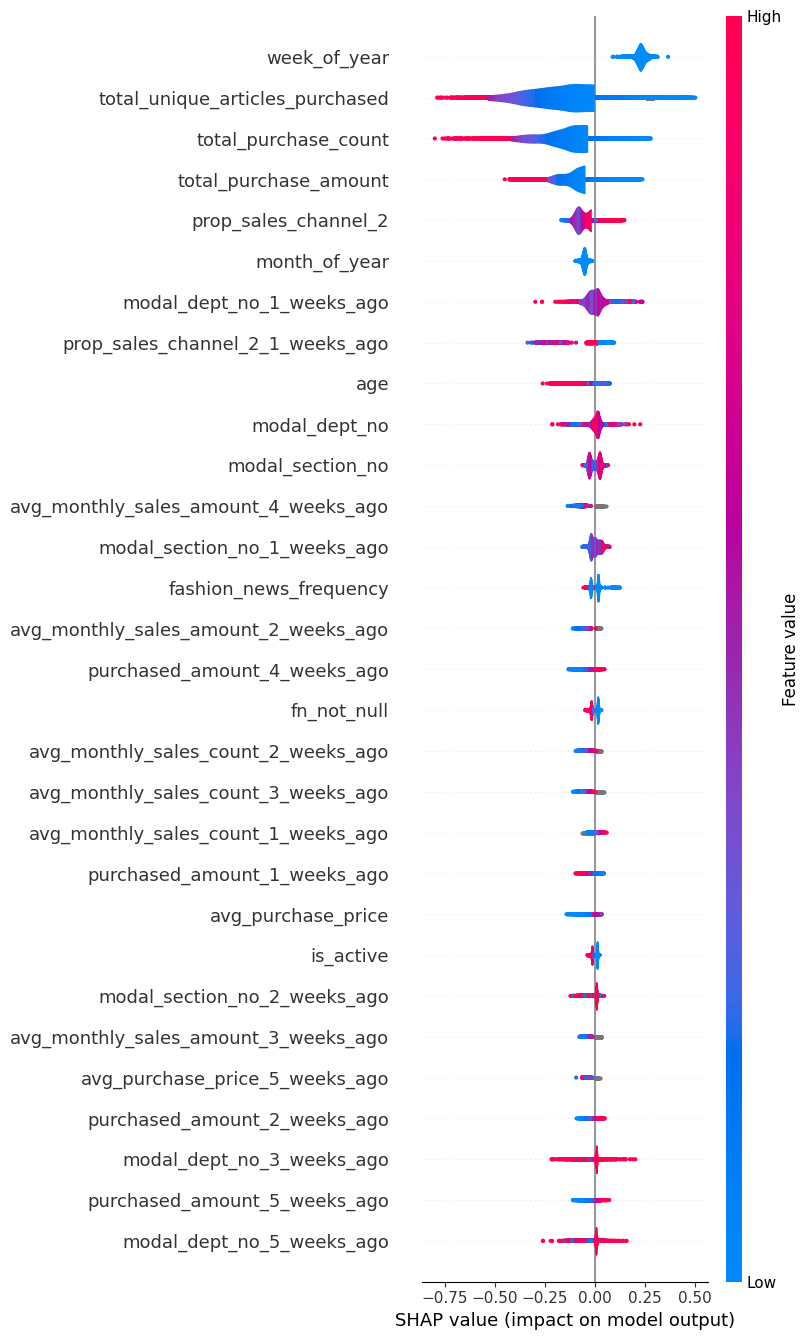
\includegraphics[width=200px]{figs/user-churn-shap.png}
% \vspace{-30pt}
\caption{\textbf{Feature Importances.} SHAP values of top 30 features ranked by importance. Note: \textit{week\_of\_year} feature shows little variability because the validation set is temporally concentrated in a few weeks.}
% \vspace{-5pt}
\label{fig:shap}
\end{figure}





\subsection{Regression Output Head Analysis}

By default, our RDL implementation uses a simple linear output head on top of the GNN embeddings. However we found that on regression tasks this sometimes led to lower than desirable performance. We found that performance on many regression tasks could be improved by modifying this output head. Instead of a linear layer, we took the output from the GNN, and fed these embeddings into a LightGBM model, which is trained in a second separate training phase from the GNN model.

The resulting model still uses an end-to-end learned GNN for cross-table feature engineering, showing that the GNN is learning useful features. Instead we attribute the weaker performance to the linear output head. We believe that further attention to the regression output head is an interesting direction for further study, with the goal of designing an output head that is performant and can be trained jointly with the GNN (unlike our LightGMB modification).

We run three experiments to study this phenomena, and attempt to isolate the output head as a problematic component for regression tasks.
%
\begin{enumerate}
    \item LightGBM trained on GNN-learned entity-level features on regression tasks. We find that this model performs better than the original GNN, suggesting that the linear output head of the GNN is suboptimal.
    \item LightGBM trained on GNN-learned entity-level features on classification tasks. We find no performance improvement, and even some degradation, compared to the original GNN model, suggesting that the observed performance boost of (1) comes not from an overall better architecture but from the correction of an innate shortcoming of the linear output head vis-a-vis regression tasks. In other words, using a LightGBM on top of the GNN is only helpful insofar as it provides a more flexible output head for regression tasks.
    \item Evaluate GNN performance after converting regression tasks to binary classification tasks with label $y = \mathbf{1}\{y_\text{regression} > 0\}$. We find that the performance gap between the data scientist models and the GNN narrow. This suggests that the GNN can learn the relevant predictive signal, but performance is affected by how the task is formulated (classification vs regression).
\end{enumerate}
%
See Tables \ref{tab:regresion analysis expt 1}, \ref{tab:regresion analysis expt 2}, \ref{tab:regresion analysis expt 3} for the results of each of these experiments. 

In Figure \ref{fig:ds main fig}, for regression tasks we report the RDL results using GNN learned features with LightGBM output head. In Table \ref{tab: regression} we report result for the basic GNN in order to avoid creating confusion for other researchers when comparing different GNN methods. We believe that Tables \ref{tab:regresion analysis expt 1}, \ref{tab:regresion analysis expt 2}, \ref{tab:regresion analysis expt 3} provide clear evidence that there is an opportunity for improvements and simplifications, which we leave to future work.


\begin{table}[t]
    \vspace{-3mm}
    \caption{Entity regression results (MAE, lower is better) on selected \relbench datasets. Training a LightGBM model on features extracted by a trained GNN leads to performance lift. This is evidence that the linear layer output head of the base GNN is suboptimal.}
    \centering
    \setlength{\tabcolsep}{3pt}
    \scriptsize
    \CatchFileDef{\tabledata}{tables/gnn_plus_lgbm_regression.tex}{}
    \begin{tabular}{llrrr}
    \toprule
    \textbf{Dataset} & \textbf{Task} & \textbf{Split} & \textbf{GNN} & \textbf{GNN+LightGBM} \\
    \midrule
    \tabledata
    \bottomrule
    \end{tabular}
    \label{tab:regresion analysis expt 1}
\end{table}

\begin{table}[t]
    \vspace{-3mm}
    \caption{Entity classification results (AUROC, higher is better, numbers bolded if withing standard deviation of best result) on selected \relbench tasks. Training a LightGBM model on features extracted by a trained GNN does not lead to performance lift, and can even hurt performance slightly. This is evidence that output head limitations hold for regression tasks only. Note, \studyOutcome uses default GNN parameters for simplicity, differing form the performance reported in the main paper.}
    \centering
    \setlength{\tabcolsep}{3pt}
    \scriptsize
    \CatchFileDef{\tabledata}{tables/gnn_plus_lgbm_classification.tex}{}
    \begin{tabular}{llrrr}
    \toprule
    \textbf{Dataset} & \textbf{Task} & \textbf{Split} & \textbf{GNN} & \textbf{GNN+LightGBM} \\
    \midrule
    \tabledata
    \bottomrule
    \end{tabular}
    \label{tab:regresion analysis expt 2}
\end{table}


\begin{table}[th]
    \vspace{-3mm}
    \caption{Entity classification results (AUROC, higher is better) on selected \relbench regression tasks, converted into classification tasks with binary label $y = \mathbf{1}\{y_\text{regression} > 0\}$. Training a LightGBM model on features extracted by a trained GNN leads to performance lift. This is evidence that the linear layer output head of the base GNN is suboptimal.}
    \centering
    \setlength{\tabcolsep}{3pt}
    \scriptsize
    \CatchFileDef{\tabledata}{tables/gnn_binarized.tex}{}
    \begin{tabular}{llrrr}
    \toprule
    \textbf{Dataset} & \textbf{Task} & \textbf{Split} & \textbf{GNN} & \textbf{Data Scientist} \\
    \midrule
    \tabledata
    \bottomrule
    \end{tabular}
    \label{tab:regresion analysis expt 3}
\end{table}

